\documentclass{article}

\usepackage{arxiv}

\usepackage[utf8]{inputenc} % allow utf-8 input
\usepackage[T1]{fontenc}    % use 8-bit T1 fonts
\usepackage{lmodern}        % https://github.com/rstudio/rticles/issues/343
\usepackage{hyperref}       % hyperlinks
\usepackage{url}            % simple URL typesetting
\usepackage{booktabs}       % professional-quality tables
\usepackage{amsfonts}       % blackboard math symbols
\usepackage{nicefrac}       % compact symbols for 1/2, etc.
\usepackage{microtype}      % microtypography
\usepackage{lipsum}
\usepackage{graphicx}

\title{ABCD Biostats Longitudinal Paper}

\author{
    Samuel W. Hawes
   \\
    Psychology; Center for Children and Families \\
    Florida International University \\
  Miami, FL 33199 \\
  \texttt{\href{mailto:shawes@fiu.edu}{\nolinkurl{shawes@fiu.edu}}} \\
   \And
    Wesley K. Thompson
    \thanks{Use footnote for providing further information about author (webpage, alternative address)---\emph{not} for acknowledging funding agencies. Optional.}
   \\
    Population Neuroscience and Genetics Lab \\
    University of California, San Diego \\
  San Diego, CA 92093 \\
  \texttt{\href{mailto:wkthompson@ucsd.edu}{\nolinkurl{wkthompson@ucsd.edu}}} \\
  }

\usepackage{color}
\usepackage{fancyvrb}
\newcommand{\VerbBar}{|}
\newcommand{\VERB}{\Verb[commandchars=\\\{\}]}
\DefineVerbatimEnvironment{Highlighting}{Verbatim}{commandchars=\\\{\}}
% Add ',fontsize=\small' for more characters per line
\usepackage{framed}
\definecolor{shadecolor}{RGB}{248,248,248}
\newenvironment{Shaded}{\begin{snugshade}}{\end{snugshade}}
\newcommand{\AlertTok}[1]{\textcolor[rgb]{0.94,0.16,0.16}{#1}}
\newcommand{\AnnotationTok}[1]{\textcolor[rgb]{0.56,0.35,0.01}{\textbf{\textit{#1}}}}
\newcommand{\AttributeTok}[1]{\textcolor[rgb]{0.77,0.63,0.00}{#1}}
\newcommand{\BaseNTok}[1]{\textcolor[rgb]{0.00,0.00,0.81}{#1}}
\newcommand{\BuiltInTok}[1]{#1}
\newcommand{\CharTok}[1]{\textcolor[rgb]{0.31,0.60,0.02}{#1}}
\newcommand{\CommentTok}[1]{\textcolor[rgb]{0.56,0.35,0.01}{\textit{#1}}}
\newcommand{\CommentVarTok}[1]{\textcolor[rgb]{0.56,0.35,0.01}{\textbf{\textit{#1}}}}
\newcommand{\ConstantTok}[1]{\textcolor[rgb]{0.00,0.00,0.00}{#1}}
\newcommand{\ControlFlowTok}[1]{\textcolor[rgb]{0.13,0.29,0.53}{\textbf{#1}}}
\newcommand{\DataTypeTok}[1]{\textcolor[rgb]{0.13,0.29,0.53}{#1}}
\newcommand{\DecValTok}[1]{\textcolor[rgb]{0.00,0.00,0.81}{#1}}
\newcommand{\DocumentationTok}[1]{\textcolor[rgb]{0.56,0.35,0.01}{\textbf{\textit{#1}}}}
\newcommand{\ErrorTok}[1]{\textcolor[rgb]{0.64,0.00,0.00}{\textbf{#1}}}
\newcommand{\ExtensionTok}[1]{#1}
\newcommand{\FloatTok}[1]{\textcolor[rgb]{0.00,0.00,0.81}{#1}}
\newcommand{\FunctionTok}[1]{\textcolor[rgb]{0.00,0.00,0.00}{#1}}
\newcommand{\ImportTok}[1]{#1}
\newcommand{\InformationTok}[1]{\textcolor[rgb]{0.56,0.35,0.01}{\textbf{\textit{#1}}}}
\newcommand{\KeywordTok}[1]{\textcolor[rgb]{0.13,0.29,0.53}{\textbf{#1}}}
\newcommand{\NormalTok}[1]{#1}
\newcommand{\OperatorTok}[1]{\textcolor[rgb]{0.81,0.36,0.00}{\textbf{#1}}}
\newcommand{\OtherTok}[1]{\textcolor[rgb]{0.56,0.35,0.01}{#1}}
\newcommand{\PreprocessorTok}[1]{\textcolor[rgb]{0.56,0.35,0.01}{\textit{#1}}}
\newcommand{\RegionMarkerTok}[1]{#1}
\newcommand{\SpecialCharTok}[1]{\textcolor[rgb]{0.00,0.00,0.00}{#1}}
\newcommand{\SpecialStringTok}[1]{\textcolor[rgb]{0.31,0.60,0.02}{#1}}
\newcommand{\StringTok}[1]{\textcolor[rgb]{0.31,0.60,0.02}{#1}}
\newcommand{\VariableTok}[1]{\textcolor[rgb]{0.00,0.00,0.00}{#1}}
\newcommand{\VerbatimStringTok}[1]{\textcolor[rgb]{0.31,0.60,0.02}{#1}}
\newcommand{\WarningTok}[1]{\textcolor[rgb]{0.56,0.35,0.01}{\textbf{\textit{#1}}}}

% Pandoc citation processing
\newlength{\csllabelwidth}
\setlength{\csllabelwidth}{3em}
\newlength{\cslhangindent}
\setlength{\cslhangindent}{1.5em}
% for Pandoc 2.8 to 2.10.1
\newenvironment{cslreferences}%
  {}%
  {\par}
% For Pandoc 2.11+
\newenvironment{CSLReferences}[2] % #1 hanging-ident, #2 entry spacing
 {% don't indent paragraphs
  \setlength{\parindent}{0pt}
  % turn on hanging indent if param 1 is 1
  \ifodd #1 \everypar{\setlength{\hangindent}{\cslhangindent}}\ignorespaces\fi
  % set entry spacing
  \ifnum #2 > 0
  \setlength{\parskip}{#2\baselineskip}
  \fi
 }%
 {}
\usepackage{calc} % for calculating minipage widths
\newcommand{\CSLBlock}[1]{#1\hfill\break}
\newcommand{\CSLLeftMargin}[1]{\parbox[t]{\csllabelwidth}{#1}}
\newcommand{\CSLRightInline}[1]{\parbox[t]{\linewidth - \csllabelwidth}{#1}\break}
\newcommand{\CSLIndent}[1]{\hspace{\cslhangindent}#1}

\usepackage{amsmath}
\newcommand{\abcd}{Adolescent Brain Cognitive Development}
\newcommand{\R}{\textsf{R}}


\begin{document}
\maketitle

\def\tightlist{}


\begin{abstract}
This is the abstract. This is the abstract. This is the abstract.
This is the abstract. This is the abstract. This is the abstract.
This is the abstract. This is the abstract. This is the abstract.
This is the abstract. This is the abstract. This is the abstract.
This is the abstract. This is the abstract. This is the abstract.
This is the abstract. This is the abstract. This is the abstract.
This is the abstract. This is the abstract. This is the abstract.
This is the abstract. This is the abstract. This is the abstract.
\end{abstract}

\keywords{
    keyword1
   \and
    keyword2
   \and
    (optional and can be removed)
  }

\hypertarget{sectioning}{%
\section{Sectioning}\label{sectioning}}

This is a section. Lorem ipsum dolor sit amet, a tincidunt turpis habitasse dapibus nam massa tempus, nullam. Lobortis pulvinar, himenaeos nisi, blandit augue. Sed euismod, mi quis lacinia semper volutpat et. Hac pulvinar etiam nascetur in vehicula fringilla nam et taciti nullam. Mattis accumsan enim ipsum. Nec mauris ultrices gravida nulla ullamcorper tempor, fermentum. Ultricies arcu a varius eu eu condimentum quam quam. Nulla lectus molestie velit mauris, sociosqu lobortis nam, cum congue ante primis. Tortor nec, egestas vel. Eu est nec ut suscipit. Urna accumsan a. A mus habitasse, morbi sem posuere, erat, platea purus sit aliquam, sodales ultricies neque lacus, rutrum.

Lorem ipsum dolor sit amet, interdum a litora ac pellentesque vel ut leo. Rhoncus sed. Tellus ullamcorper efficitur mauris et. Sollicitudin rutrum orci, sed fermentum urna diam, nec platea fusce massa. Tortor suspendisse quam lobortis senectus semper pellentesque, in enim. Justo eleifend ante urna sit elementum elementum nascetur, nec lacus. Amet at congue ridiculus. Eget taciti condimentum sem nunc. Libero elementum tempus habitasse eleifend cursus sed eleifend ultricies. Viverra suscipit eu integer ipsum. Purus sed mollis sed, sed dignissim nisi torquent risus? Praesent sit sed tincidunt turpis nisl ornare ipsum. Ornare aenean ad morbi mauris arcu, sociosqu. Eu posuere ridiculus purus, ante. Vestibulum, himenaeos eu nulla dolor ante dignissim at neque, et. Imperdiet fringilla class commodo leo, tempus at non semper. Scelerisque faucibus faucibus eu habitasse pellentesque.

\hypertarget{subsection}{%
\subsection{Subsection}\label{subsection}}

This is a subsection. Lorem ipsum dolor sit amet, convallis et class. Hendrerit nec sed commodo at eros feugiat ut ac at! Tincidunt et ex, dapibus. Pretium id sem ac netus et. Scelerisque velit aenean congue dui nisl et? Turpis non vitae nec porttitor ac at, montes suscipit aliquam parturient lectus in. Non conubia justo parturient ut vitae nisl rhoncus nullam parturient diam justo. Amet sit magna blandit est eleifend dictumst et eros. Ante mauris, odio in nec sagittis euismod hac. Ornare luctus lacinia aliquet sed integer cum suscipit finibus, platea velit. Ex potenti quis pharetra et quisque. Nisl malesuada rhoncus ligula et, tincidunt sit. Vitae, himenaeos blandit sed fringilla volutpat, nascetur et consectetur.

Lorem ipsum dolor sit amet, sed habitasse gravida pellentesque suspendisse imperdiet nam purus consequat integer sapien arcu. Inceptos nibh metus, laoreet. Accumsan sem turpis tincidunt felis id id vitae sed, lectus ultrices morbi feugiat non placerat. Class est iaculis, aenean, augue gravida gravida. Ultricies sed litora aptent semper aliquam ornare sed dictum ac inceptos quisque sodales. Nostra, lorem nisl at purus a, eleifend, ut vel eu. Conubia torquent libero, dignissim lorem sapien duis. Massa sociis enim tempor condimentum, vitae nibh dolor pellentesque. Scelerisque tellus pellentesque mi suspendisse aptent habitant tincidunt per metus. Nec adipiscing pulvinar sodales, nam, ac a habitant, libero class sapien nulla. Nec iaculis tempus porta. Potenti feugiat, mus pharetra. Amet facilisi a velit, integer, ex eget, nibh in.

\hypertarget{subsubsection}{%
\subsubsection{Subsubsection}\label{subsubsection}}

This is a subsubsection. Lorem ipsum dolor sit amet, feugiat et erat vivamus, hac. Mauris mauris nisl. Lacus, pretium amet ex ante amet quis vitae nam cum, eu justo. In in. Ac consequat massa ante pellentesque ultricies justo. Ut nulla metus, phasellus, risus sapien sed dis. Id mauris pulvinar ut ipsum cubilia eros habitasse. Morbi commodo sed pellentesque aliquam maximus.

Lorem ipsum dolor sit amet, magnis vel convallis venenatis fermentum, magnis. Elit donec vehicula egestas dignissim aenean sit quis et sit massa. Et nam. Ex et gravida mauris sed sed, ut eros ac elit ac. Vestibulum pellentesque eros? Egestas pulvinar placerat, convallis viverra faucibus consequat in scelerisque. Ipsum ex, felis. Ipsum eget arcu dignissim. Class sed penatibus et auctor. Vehicula sed, netus sociis.

\hypertarget{paragraph}{%
\paragraph{Paragraph}\label{paragraph}}

This is a paragraph. Lorem ipsum dolor sit amet, curabitur laoreet ultricies eros proin et condimentum rutrum aptent. Nullam amet at, ac risus, egestas finibus eu. Luctus in ut elementum. Aenean tellus, felis magna et, enim ac velit augue donec. Porta ac dictumst erat ex arcu nec et porttitor ut. Vitae vestibulum a aptent sed, a, aliquam neque sed, interdum libero, fermentum. Convallis pellentesque congue sed iaculis amet rhoncus etiam ligula diam vel neque. Amet a cum phasellus, tincidunt erat magnis velit non in. Quis eu facilisis venenatis venenatis. Tempor netus amet ac nostra arcu magnis sed in quis eu. Eget, porta ante, gravida praesent pretium lacus eros non.

Lorem ipsum dolor sit amet, hendrerit duis at sapien montes pellentesque imperdiet nec lorem posuere in. Pellentesque elit nec mus nec. In potenti natoque, consectetur augue. Rhoncus eleifend eu ante felis sapien. Cum aliquam ut aliquam quam, varius velit, mauris. Aliquam consectetur curabitur magna, venenatis, justo pellentesque etiam auctor maecenas. Et elementum a eros, posuere maximus sed consequat ac vivamus. Rhoncus sed, eu imperdiet luctus lacus ipsum. Volutpat nibh aliquet eros lacus, mattis turpis blandit. Lorem finibus vivamus neque mattis ante. Ullamcorper pellentesque nulla ligula mus malesuada ac torquent at sed semper.

\hypertarget{pandoc}{%
\section{(Pandoc) Markdown syntax}\label{pandoc}}

\hypertarget{basic-formatting}{%
\subsection{Basic formatting}\label{basic-formatting}}

Text can be \textbf{bold}, \emph{italic}, or \texttt{verbatim} (e.g., for code).

\medskip\noindent This is a quotation:

\begin{quote}
\emph{This is an infamous quote.}

\smallskip\sffamily\footnotesize --- The Author
\end{quote}

\medskip\noindent Explicit URLs and email addresses are automatically converted to clickable links, e.g., \url{https://abcdstudy.org} and \href{mailto:janosch@ucsd.edu}{\nolinkurl{janosch@ucsd.edu}}. Links can also be shown with alternative text, e.g., The ABCD study's \href{https://abcdstudy.org}{website} and Janosch's \href{mailto:janosch@ucsd.edu}{email address}.

One can also use \LaTeX~syntax directly if one has or wants to, like the \texttt{\textbackslash{}medskip\textbackslash{}noindent} above.

\hypertarget{footnotes}{%
\subsection{Footnotes}\label{footnotes}}

Footnotes can be added like this.\footnote{This is a footnote.}

\hypertarget{lists}{%
\subsection{Lists}\label{lists}}

This is an \emph{unordered} list:

\begin{itemize}
\tightlist
\item
  first item
\item
  second item

  \begin{itemize}
  \tightlist
  \item
    first subitem
  \item
    second subitem

    \begin{itemize}
    \tightlist
    \item
      first subsubitem
    \item
      second subsubitem
    \end{itemize}
  \end{itemize}
\item
  third item
\end{itemize}

\noindent This is an \emph{ordered} list:

\begin{enumerate}
\def\labelenumi{\arabic{enumi}.}
\tightlist
\item
  first item
\item
  second item
\item
  third item
\item
  fourth item
\item
  fifth item
\item
  sixth item
\item
  seventh item
\item
  eighth item
\item
  ninth item
\item
  tenth item

  \begin{enumerate}
  \def\labelenumii{\roman{enumii}.}
  \tightlist
  \item
    first subitem
  \item
    second subitem
  \item
    third subitem
  \item
    fourth subitem
  \item
    fifth subitem
  \item
    sixth subitem
  \item
    seventh subitem
  \item
    eighth subitem
  \item
    ninth subitem
  \item
    tenth subitem
  \item
    eleventh subitem

    \begin{enumerate}
    \def\labelenumiii{\alph{enumiii}.}
    \tightlist
    \item
      first subsubitem
    \item
      second subsubitem
    \item
      third subsubitem
    \end{enumerate}
  \end{enumerate}
\item
  eleventh item
\end{enumerate}

\hypertarget{citations}{%
\subsection{Citations}\label{citations}}

Citations can be added using the following syntax:

\begin{itemize}
\tightlist
\item
  \texttt{{[}@citation1{]}} / \texttt{{[}@citation2;\ @citation3{]}} for parenthetical citations.\footnote{Prefixes and suffixes can be added to parenthetical citation, e.g., \texttt{{[}cf.,\ @citation1{]}}.}
\item
  \texttt{@citation4} for in-text citations.
\end{itemize}

This is what one paper says (see Hadash et al. 2018, for an overview). This is what two other say (Kour and Saabne 2014b, 2014a). Hadash et al. (2018) said more.

\hypertarget{mathematical-notation}{%
\subsection{Mathematical notation}\label{mathematical-notation}}

Math is based on \LaTeX~syntax.\footnote{See, e.g., \url{https://en.wikibooks.org/wiki/LaTeX/Mathematics} or \url{https://www.overleaf.com/learn/latex/mathematical_expressions}.} To display math inline, one has to enclose mathematical expressions in \texttt{\$...\$}, e.g., \(\sum_{n=1}^{10} n^2\). To add an equation, one can utilize \LaTeX~equation environments:

\begin{equation}
Y_i = \beta_0 + \beta_1 X_i + \epsilon_i
\label{eq:regression}
\end{equation}

\hypertarget{r-markdown-syntaxelements}{%
\section{R Markdown syntax/elements}\label{r-markdown-syntaxelements}}

\hypertarget{code}{%
\subsection{Code}\label{code}}

One can embed arbitrary \textsf{R}~code\footnote{A number of other programming languages are also supported, see \url{https://bookdown.org/yihui/rmarkdown/language-engines.html}.} anywhere in the document like ``the square root of 36 is 6.'' Furthermore, one can use ``code chunks'' to execute bigger chunks of \textsf{R}~code and have the results displayed in the document (or not\footnote{For an overview of different chunk options which determine how code chunks are displayed in the resulting document, see \url{https://yihui.org/knitr/options/}.}).

\footnotesize

\begin{Shaded}
\begin{Highlighting}[]
\CommentTok{\# select variables}
\NormalTok{y }\OtherTok{\textless{}{-}}\NormalTok{ iris}\SpecialCharTok{$}\NormalTok{Species}
\NormalTok{x }\OtherTok{\textless{}{-}}\NormalTok{ iris}\SpecialCharTok{$}\NormalTok{Sepal.Length}

\CommentTok{\# print regression model}
\FunctionTok{glm}\NormalTok{(y}\SpecialCharTok{\textasciitilde{}}\NormalTok{x, }\AttributeTok{family =} \StringTok{\textquotesingle{}binomial\textquotesingle{}}\NormalTok{)}
\end{Highlighting}
\end{Shaded}

\begin{verbatim}
Call:  glm(formula = y ~ x, family = "binomial")

Coefficients:
(Intercept)  
    -27.829  
          x  
      5.176  

Degrees of Freedom: 149 Total (i.e. Null);  148 Residual
Null Deviance:      191 
Residual Deviance: 71.84    AIC: 75.84
\end{verbatim}

\normalsize

\hypertarget{figures}{%
\subsection{Figures}\label{figures}}

Code chunks can also be used to embed plots generated with \textsf{R}~(or other programming languages). The appearance of figures in the output document can be modified using chunk options.\footnote{See, e.g., \url{http://zevross.com/blog/2017/06/19/tips-and-tricks-for-working-with-images-and-figures-in-r-markdown-documents}.} For example, the following prints a figure that takes up 75\% of the column width. It's set in a floating environment, so might not appear at this exact location.

\begin{figure}

{\centering 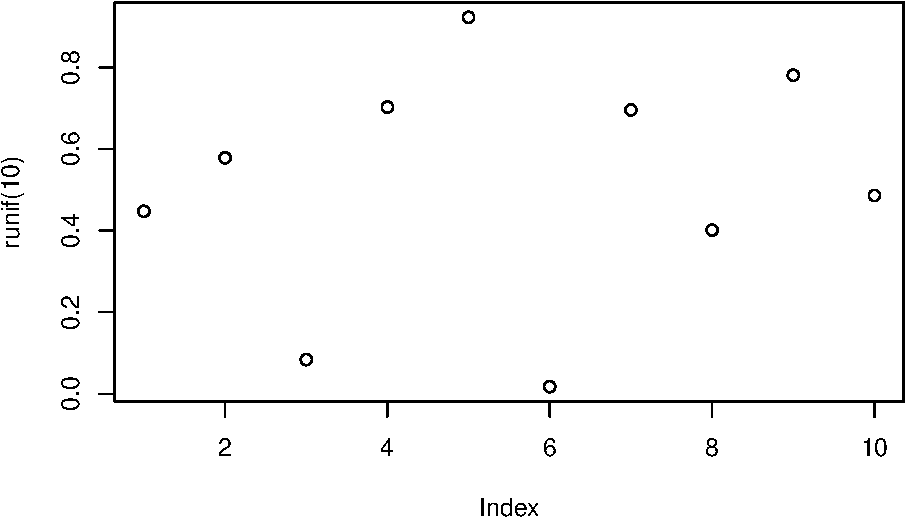
\includegraphics[width=0.75\linewidth]{paper_files/figure-latex/fig-75percent-1} 

}

\caption{A figure.}\label{fig:fig-75percent}
\end{figure}

\medskip\noindent While it possible to use standard Markdown syntax to include locally stored images, it's suggested to also use code chunks for these images. This makes it easy to format an image's appearence, add figure captions, and reference figures throughout the document (see below). The following figure is using a local image.

\hypertarget{cross-references}{%
\subsection{Cross-references}\label{cross-references}}

Using the Bookdown extension of \textsf{R}~Markdown, it is possible to embed cross-references to different elements of the document.\footnote{See \url{https://bookdown.org/yihui/bookdown/cross-references.html}.}

\begin{itemize}
\tightlist
\item
  \texttt{\textbackslash{}@ref(section-id)} to reference sections, e.g., see Section \ref{pandoc}.
\item
  \texttt{\textbackslash{}@ref(fig:plot-name)} to reference figures, e.g., see Figure \ref{fig:fig-75percent}.
\item
  \texttt{\textbackslash{}@ref(eq:equation-name)} to reference equations, e.g., see Equation \eqref{eq:regression}.
\end{itemize}

\hypertarget{random-tips-and-tricks}{%
\section{Random tips and tricks}\label{random-tips-and-tricks}}

\begin{itemize}
\tightlist
\item
  To make on-the-fly changes to the layout

  \begin{itemize}
  \tightlist
  \item
    use \texttt{header\_includes} in the YAML header to add code to the \LaTeX~preamble or
  \item
    put a modified class file in the same directory as the \texttt{.Rmd} file.
  \end{itemize}
\item
  To eliminate ``overfull lines/boxes''

  \begin{itemize}
  \tightlist
  \item
    modify \LaTeX's \texttt{\textbackslash{}emergenystretch} parameter by including, e.g., \texttt{\textbackslash{}setlength\{\textbackslash{}emergencystretch\}\{8em\}} in the \texttt{.Rmd} file before the first overful box.
  \end{itemize}
\item
  To have URLs in figure captions be displayed with colored links

  \begin{itemize}
  \tightlist
  \item
    use \texttt{\textbackslash{}\textbackslash{}url\{\}} around the URL.
  \end{itemize}
\end{itemize}

\hypertarget{summary}{%
\section{Summary}\label{summary}}

This document gave a brief introduction on how to use R Markdown to generate reports in PDF format. For more thorough information on how to use \textsf{R}~Markdown, see the following web resources:

\begin{itemize}
\tightlist
\item
  \href{https://bookdown.org/yihui/rmarkdown/}{\textsf{R}~Markdown guide}
\item
  \href{https://bookdown.org/yihui/rmarkdown-cookbook/}{\textsf{R}~Markdown cookbook}
\item
  \href{https://rmd4sci.njtierney.com/}{\textsf{R}~Markdown for scientists}
\item
  \href{https://bookdown.org/yihui/bookdown/}{Bookdown book}
\end{itemize}

\hypertarget{references}{%
\section*{References}\label{references}}
\addcontentsline{toc}{section}{References}

\hypertarget{refs}{}
\begin{CSLReferences}{1}{0}
\leavevmode\hypertarget{ref-hadash2018estimate}{}%
Hadash, Guy, Einat Kermany, Boaz Carmeli, Ofer Lavi, George Kour, and Alon Jacovi. 2018. {``Estimate and Replace: A Novel Approach to Integrating Deep Neural Networks with Existing Applications.''} \emph{arXiv Preprint arXiv:1804.09028}.

\leavevmode\hypertarget{ref-kour2014fast}{}%
Kour, George, and Raid Saabne. 2014a. {``Fast Classification of Handwritten on-Line Arabic Characters.''} In \emph{Soft Computing and Pattern Recognition (SoCPaR), 2014 6th International Conference of}, 312--18. IEEE.

\leavevmode\hypertarget{ref-kour2014real}{}%
---------. 2014b. {``Real-Time Segmentation of on-Line Handwritten Arabic Script.''} In \emph{Frontiers in Handwriting Recognition (ICFHR), 2014 14th International Conference on}, 417--22. IEEE.

\end{CSLReferences}

\bibliographystyle{unsrt}
\bibliography{references.bib}


\end{document}
